\documentclass[iop]{emulateapj}

\begin{document}

\title{Disk Evolution in the Merger of the Milky Way and Andromeda}

\author{Ryan Hofmann}
\affil{Department of Astronomy, University of Arizona}

\begin{abstract}
Galactic disk evolution is driven by both internal and external forces. Understanding this process and the forces involved is necessary for a complete description of galaxy formation and evolution. In this paper, I examine how the disks of the Milky Way and Andromeda warp and thicken throughout their merger; I also show empirically the relationship between disk thickness and velocity dispersion and discuss how the disks are heated by gravitational interactions. Such relations can be applied, with some assumptions, to real galaxies, giving some indication of their age and evolutionary history to corroborate other methods, as well as helping to constrain this and future models of interactions between disk galaxies. I observe tidal warping and streaming in the simulation, and find that the disk thickness and velocity dispersion can be described at early times by a linear relation, with slope $m \sim 46$ km s$^{-1}$ kpc$^{-1}$ for Andromeda, and less than half that value for the Milky Way. This difference is likely a reflection of the smaller stellar mass of the Milky Way; this and my other observations are mostly consistent with theoretical predictions.
\end{abstract}

\section{Introduction}
The disks of spiral galaxies are dynamic systems, influenced both by external forces and by internal kinematics, and as such, they can provide an excellent record of the history and current state of galaxies like our own Milky Way. By studying the evoution of disk morphologies in simulations of galaxy interactions, we can gain a better understanding of what causes real galactic disks to evolve as they do; conversely, we can use the current properties of disks with other information to determine the evolutionary history of galaxies.

Galactic disks typically undergo two types of evolution: they grow thicker as time passes; and they can warp, bend, and twist into various shapes. The thickening of a disk with age can be understood in terms of internal kinematics. As the disk is made up of many stars, essentially point masses, each point mass can scatter off of others nearby, with most of the effect probably being due to a combination of molecular clouds, spiral density waves, and external heating from minor merger events \citep{Mer00}. Because stars interact solely through gravity, rather than being subject to viscous forces as in the thin gas disk, the overall trend is for the disk to puff up as it ages. Typically, a disk galaxy like the Milky Way will have two or more disks, each dominated by stars around a certain age: the thin disk is dominated by young stars that have not had time to disperse, and the thick disk is dominated by older stars. Each component can be fit by a separate Miyamoto-Nagai exponential profile with its own scale height; scale height is the distance above or below the disk at which the density drops to $\frac{1}{e} \approx 0.368$ of the maximum. In this paper, I use the spread of the density function as a proxy for the scale height, assuming that $\sigma_z \sim h_s$.

The more noticeable way for a disk to change is through gravitational interactions with other galaxies. There are two main types of disk deformations: warps and tidal tails. The Milky Way's disk has a slight warp: one side curves up with respect to the disk plane, while the other side bends slightly down. This warping is caused by gravitational tidal forces perpendicular to the disk plane; in the case of the Milky Way, the culprits are the Magellanic Clouds. Specifically, as the Magellanic Clouds orbit the Milky Way, they excite a resonance in the dark matter halo, causing the gravitational potential to oscillate up and down. This oscillation causes the Milky Way's disk to "flap" in a manner reminescent of a table cloth blowing in the wind.

Tidal tails are a much more noticeable disk distortion, and are typically caused by tidal forces acting in the plane of the disk. During the mid-1900's, it was believed that gravitational tides alone could not explain the long, narrow features called tidal tails. Then, in 1972, the Toomre brothers \citep{Too72} showed through N-body simulations that gravity could indeed cause tidal tails, especially if the two galaxies were moving in the same direction as they rotated (prograde). These tidal tails typically take the form of a two-armed spiral, caused by mass spilling over the L1 and L2 Lagrange points of the system. The fate of the material drawn out into these tidal tails depends on the relative masses and velocities of the interacting galaxies. At high mass and low velocity, the material infalls, either into the second galaxy or back into the first. At the reverse extreme, the tails have enough energy to escape the system. In most cases, at least some of the material from the tails ends up as stellar streams in the halo of the merged object.

Of course, the majority of cases in which two similar disk galaxies interact involve both warping and tidal tail formation in both disks, to varying degrees depending on the mass and rotation rate of each. There are many possible variations on this theme, some of which are observed in the real world. In order to better understand not only how galaxies are built, but also what factors influence galactic mergers and cluster dynamics, it is helpful to simulate the interaction of galaxies in a well-known system, such as the Milky Way - Andromeda pair, and by analyzing the behavior of these galaxies with realistic inputs, extrapolate to other systems in the nearby universe.

\section{This Project}
In this project, I am analyzing a simulation of the Milky Way/Andromeda merger to determine how the disks of the two main galaxies evolve over time. In particular, I am looking for an empirical relationship between the disk thickness $h$ and velocity dispersion $v_z$. I will relate this relationship to the disk heating during quiescent periods of the encounter. I also aim to create, using the simulation data, an animated sequence showing the evolution of the galaxies' disks in pseudo-3D, i.e. plotting the disk as a 2D histogram both face-on and edge-on next to one another. In this sequence, the warping and tidal tails are clearly visible.

\section{Methods}
For this project, I am using a collisionless N-body simulation from \citet{van12}, including only stars and dark matter. The simulation was calculated using the GADGET-3 hydrodynamics code \citep{Spr05}. Because gas comprises only a small fraction of each galaxy's mass, it is ignored. The coordinates are Galactocentric, with the Milky Way starting at rest at the origin at $t=0$. The parameters of each galaxy were taken from the literature. The simulation starts at the present epoch and runs until $t=10$ Gyr into the future.

To analyze the simulation, I have written several pieces of Python code. I used the homework examples for reading a file and calculating the center of mass as a starting point. From there, the code rotates the coordinate system so that the z-axis is aligned with the angular momentum vector, using the 3D rotation matrix :

\begin{equation}
R = I + {\lbrack v \rbrack}_\times + {\lbrack v \rbrack}_\times^2 \frac{1-c}{s^2}
\end{equation}

where $I$ is the $3\times3$ identity matrix, $v = a \times b$ for unit vectors $a$ and $b$, $s = ||v||$ is the sine of the angle, $c = a \cdot b$ is the cosine of the angle, and ${\lbrack v \rbrack}_\times$ is the skew-symmetric cross-product matrix of $v$,

\[
{\lbrack v \rbrack}_\times \equiv \left[ \begin{array}{ccc}
0 & -v_3 & v_2 \\
v_3 & 0 & -v_1 \\
-v_2 & v_1 & 0 \end{array} \right]
\]

Once the coordinates have been rotated, the disk can be plotted as a 2D histogram, either face-on or edge-on. In batch mode, the program does this for each in a series of snaps from the simulation and saves the plots as PNG files, which can be combined into a movie with ffmpeg.

I also wrote a more advanced version of this program. It plots the disk face-on and edge-on on one side, and on the other side are histograms of $z$ and $v_z$ for the disk particles. The main program loops over a range of snaps, creates a PNG plot for each snap, and ends by plotting $\sigma_{v_z}$ against $\sigma_z$ over the range of snaps. This plot is saved as both a PNG plot and a text file containing three columns: time in Myr, $\sigma_z$ in kpc, and $\sigma_{v_z}$ in km/s.

\section{Results}
A sample plot from my program is shown in Figure \ref{fig:m31stats}. The timestep shown is \#315, $~500$ Myr after the first close encounter between the Milky Way and Andromeda.

\subsection{Tidal Spirals}
One immediately noticeable feature of Figure \ref{fig:m31stats} is the prominent pair of spiral arms. These arms are not density wave structures like normal spiral arms; instead, they are the direct result of the gravitational tidal interaction between the main galaxies. The formation of these structures, as first demonstrated in \citet{Too72}, is a direct consequence of tidal forces in a prograde encounter. Because the encounter is not coplanar with the disks, the tidal tails extend above and below the disk plane.

\begin{figure*}[t]
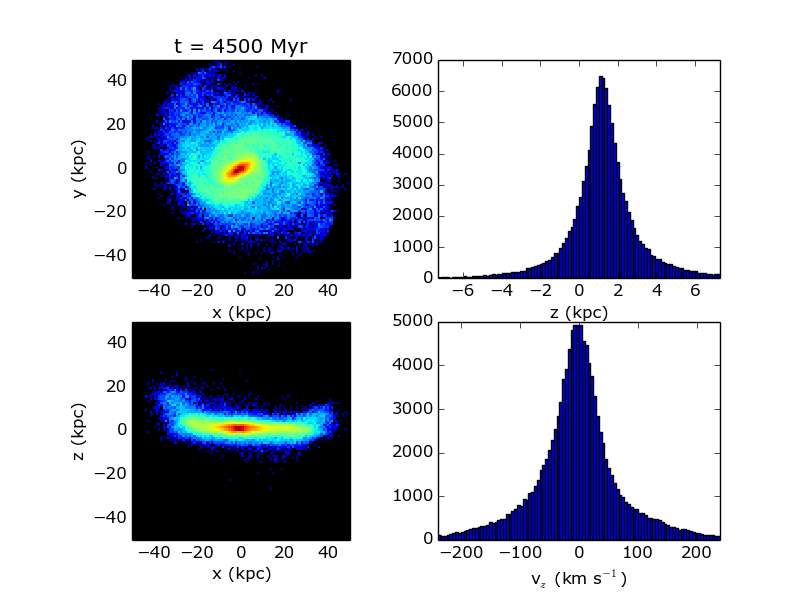
\includegraphics[width=18cm]{../M31_000_599_stats/M31_315.png}
\caption{Sample plot of M31 after first pericenter, snap \#315. Top left: face-on plot showing two tidal arms; time since the present is written at the top. Bottom left: edge-on plot. Both are density plots of disk particles only. Top right: distribution of particles about disk plane, with standard deviation $\sigma_z$. Bottom right: distribution of vertical particle velocities, with standard deviation $\sigma_{v_z}$.}
\label{fig:m31stats}
\end{figure*}

\begin{figure*}[t]
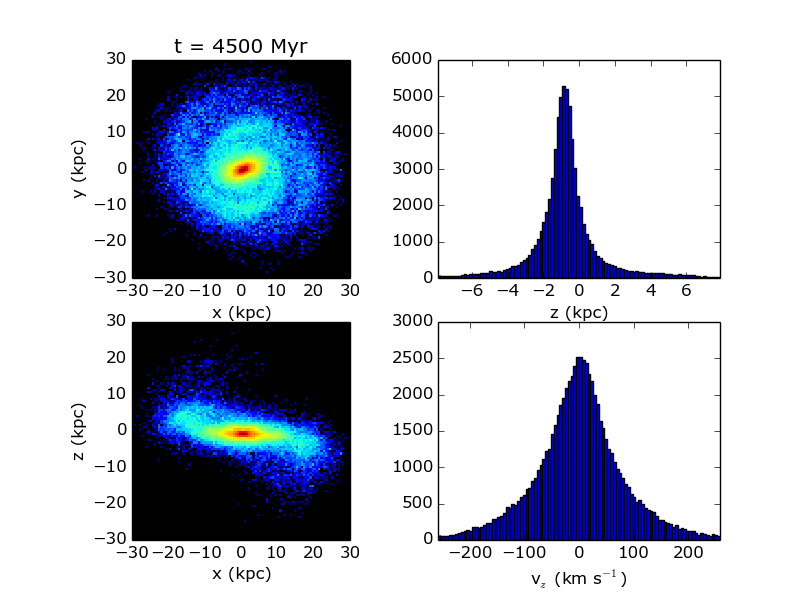
\includegraphics[width=18cm]{../MW_000_599_stats/MW_315.png}
\caption{Sample plot of MW after first pericenter, snap \#315. Top left: face-on plot showing two tidal arms; time since the present is written at the top. Bottom left: edge-on plot. Both are density plots of disk particles only. Top right: distribution of particles about disk plane, with standard deviation $\sigma_z$. Bottom right: distribution of vertical particle velocities, with standard deviation $\sigma_{v_z}$.}
\label{fig:mwstats}
\end{figure*}

\subsection{Disk Thickening}
Figure \ref{fig:m31disp} shows the evolution of $\sigma_{v_z}$ and $\sigma_z$ in M31 over the course of the merger. During the first part of the simulation, before the first pericenter, the two dispersions increase almost linearly with one another. The data for the Milky Way are similar, but of lower quality, most likely due to the smaller number of particles. Fitting a straight line to the early part of the graph and comparing between the two galaxies, it can be seen that the slope for M31 is more than twice that for the Milky Way.

\begin{figure*}[c]
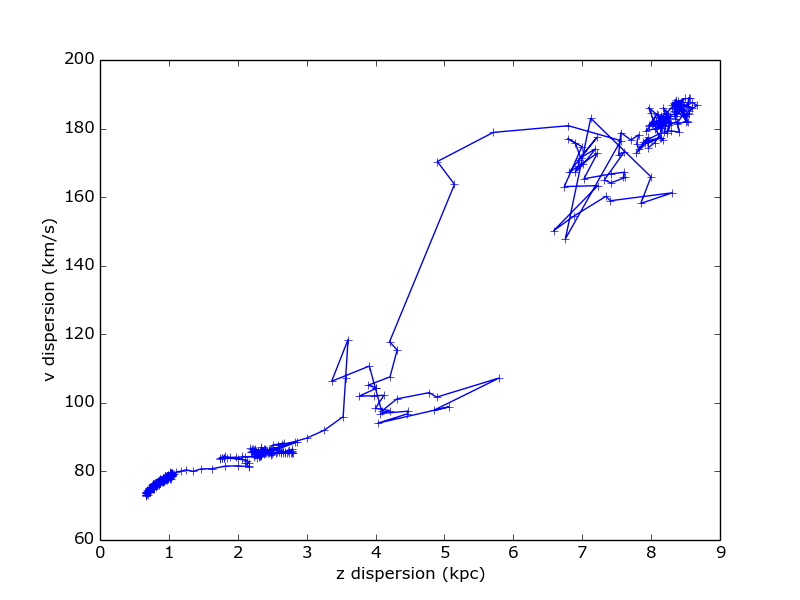
\includegraphics[width=12cm]{../MW_000_599_stats/MW_dispersions.png}
\caption{Dispersions in position and velocity in z direction for the Milky Way.}
\label{fig:mwdisp}
\end{figure*}

\begin{figure*}[c]
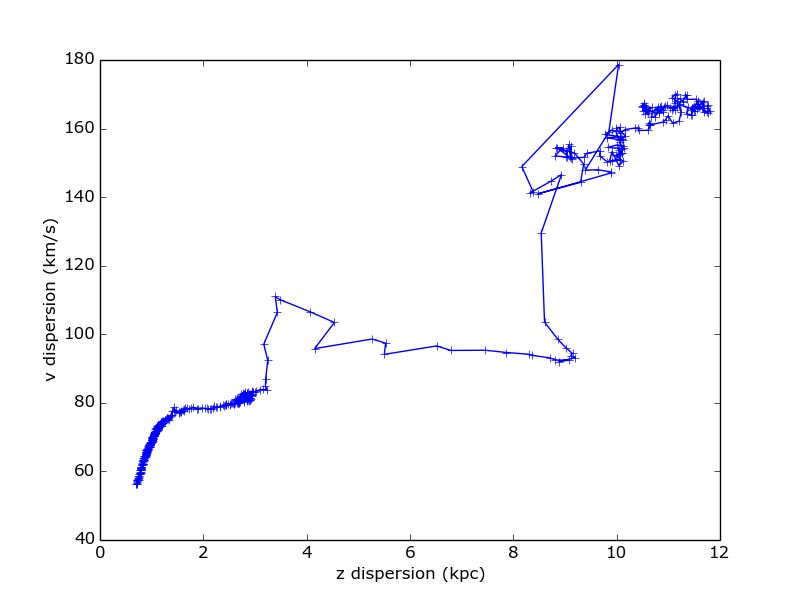
\includegraphics[width=12cm]{../M31_000_599_stats/M31_dispersions.png}
\caption{Dispersions in position and velocity in z direction for M31.}
\label{fig:m31disp}
\end{figure*}

Another interesting thing that I noticed in Figure \ref{fig:m31disp} is that during the first pericenter, $\sigma_z$ increases dramatically, while $\sigma_{v_z}$ increases more steadily. Both values skyrocket during the second and third pericenters, then level off as the merged object settles down.

\section{Discussion}
\subsection{Tidal Effects}
As can be seen in Figure \ref{fig:m31stats}, M31's disk is undergoing both kinds of tidal distortion: warping and tidal tails. The two effects overlap, producing tidal tails that curve upwards from the disk plane. Comparing with Figure \ref{fig:mwstats} for the Milky Way, it is immediately apparent that the two galaxies are experiencing different warping modes. This is even more apparent in the full sequences: while the tidal arms of M31 seem to oscillate gracefully up and down, the disk of the Milky Way warps asymmetrically, then the pattern seems to remain frozen - the galaxy rotates, but the warps stay in place. This difference is likely due to the difference in disk mass, as well as to the strength of the external gravitational force exciting the oscillations for each galaxy.

Intriguingly, for several snaps after the first pericenter, the tidal arms of the Milky Way merge in the inner disk to form a ring. This may have implications for theories of ring formation in non-isolated galaxies.

\subsection{Kinematics}
As can be seen from the dispersion plots, the positional distribution is the first to spread following a pericenter. Logically, this makes sense just from the statistics plots: some of the stars in the disk have been drawn out of the disk plane by the tidal interactions, and the close pass also injected a lot of energy into the disk, causing it to expand in a similar manner to a heated gas. The time of each close pass is clearly visible as where $\sigma_z$ suddenly and rapidly increases.

\section{Conclusion}
I analyzed an N-body simulation of the Milky Way - Andromeda merger, looking for effects of tidal interactions and disk thickening. Using a custom Python code, I plotted each galaxy with their statistics for a range of snapshots, then put all the plots together into a movie. I also plotted the relationship between $\sigma_z$ and $\sigma_{v_z}$ for each galaxy and determined a linear proportionality for the first $\sim 140$ Myr; the proportionality constant was more than twice as large for M31 as for the Milky way. Tidal tails and disk warping are observed in both galaxies, with the warp oscillation mode differing between the two galaxies. Most differences in the appearance and behavior of the two galaxies can be ascribed to the difference in disk mass and the strength of the gravitational tidal forces.

Due to time constraints, I was unable to perform much in-depth analysis of the data here presented. If I had more time, I would have liked to achieve a more quantitative description of the disk heating and mass loss through tidal streaming. Other steps might include fine-tuning the code to minimize jitter between frames.

\begin{thebibliography}{}
\bibitem[Merrifield(2000)]{Mer00} Merrifield, M. R. 2000, ASP Conference Series, 230, 221
\bibitem[Springel(2005)]{Spr05} Springel, V. 2005, MNRAS, 364, 1105
\bibitem[Toomre and Toomre(1972)]{Too72} Toomre A., Toomre J. 1972, \apj, 178, 623
\bibitem[van der Marel et al.(2012)]{van12} van der Marel, R. P., Besla, G., Cox, T. J., Sohn, S.T., \& Anderson, J. 2012, \apj, 753, 9
\end{thebibliography}

\end{document}
